\documentclass[10pt]{beamer}
\usetheme{Madrid}
\usepackage{booktabs}
\usepackage{graphicx}
\usepackage[T1]{fontenc}
\usepackage{tikz}
\usetikzlibrary{arrows.meta}
\setbeamertemplate{navigation symbols}{}
% To view speaker notes, uncomment the next line (adds note pages):
% \setbeameroption{show notes}
\tikzset{
  box/.style={draw, rounded corners, align=center, text width=2.3cm, minimum height=0.9cm, font=\scriptsize},
  kuser/.style={box, fill=blue!15}, kagent/.style={box, fill=green!25},
  kdata/.style={box, fill=black!8}, kdanger/.style={box, fill=red!25},
  koutput/.style={box, fill=orange!25}, kdecision/.style={box, fill=yellow!30},
  kguard/.style={box, fill=violet!25},
  flow/.style={-{Stealth[length=2mm]}, thick},
}
% ======================= EDIT YOUR DETAILS =======================
\newcommand{\studentname}{Aflah Muhammed P}
% Change the university roll/registration number:
\newcommand{\rollno}{TVE23CSXXX}
% Change your class roll number:
\newcommand{\rollclass}{Roll No: XX}
% Change your guide name:
\newcommand{\guidename}{Prof. Guide Name}
% Change department / college / short-institute if needed:
\newcommand{\deptname}{Department of Computer Science and Engineering}
\newcommand{\collegename}{College of Engineering Trivandrum}
\newcommand{\shortinst}{CET}
% Change the seminar date:
\newcommand{\seminardate}{\today}
% =================================================================
\title[B.Tech Seminar]{How Large Language Models Turn Goals into Plans: A Beginner's Guide to the LLM Planning Survey}
\subtitle{Based on: Large Language Models for Planning: A Comprehensive and Systematic Survey (arXiv:2505.19683, 2025)}
\author[\studentname\ (\shortinst)]{\studentname \\ \small \rollno \\ \small \rollclass \\ \small Guide: \guidename}
\institute[]{\deptname \\ \collegename}
\date{\seminardate}
\begin{document}
\begin{frame}[plain]
  \titlepage
\end{frame}
\begin{frame}{Table of Contents}
  \tableofcontents
\end{frame}
\section{Introduction}
\begin{frame}{Introduction}
\begin{itemize}
  \item Planning means breaking a big goal into an ordered set of steps
  \item Humans plan naturally; we want AI agents to plan reliably too
  \item Large Language Models can read a goal and propose action steps
  \item This 2025 survey organizes hundreds of LLM planning methods clearly
  \item It groups methods into three families and reviews how we test them
  \item Goal today: understand the landscape without heavy math or jargon
\end{itemize}
\end{frame}
\note{Welcome everyone. Today we will talk about how AI systems built on large language models can take a goal and turn it into a step-by-step plan. Don't worry if you're new to this, because I'll define every term as we go. By the end you'll have a clear map of the whole field.}
\section{Literature Survey}
\begin{frame}{Literature Survey / Background}
  \small
  \begin{tabular}{@{}p{2.7cm}p{2.3cm}p{5.6cm}@{}}
    \toprule
    \textbf{Title} & \textbf{Author} & \textbf{Summary} \\
    \midrule
    TravelPlanner: A Benchmark for Real-World Planning & Xie et al., 2024 & Real-world travel planning benchmark; even GPT-4 passes only 0.6 percent, showing planning is genuinely hard for LLMs. \\
    \addlinespace
    Tree of Thoughts: Deliberate Problem Solving with LLMs & Yao et al., 2023 & Lets a model explore several reasoning branches like a tree, backtracking to find a better plan. \\
    \addlinespace
    LLM+P: Empowering LLMs with Optimal Planning & Liu et al., 2023 & Translates a task into formal PDDL so a classical planner can solve it reliably and optimally. \\
    \addlinespace
    \bottomrule
  \end{tabular}
\end{frame}
\note{Before we dive in, here are three papers that set the stage. TravelPlanner is a benchmark that showed even a powerful model like GPT-4 struggles badly with real planning. Tree of Thoughts and LLM+P are two influential methods we'll meet again later, one that searches through ideas and one that hands the problem to a classical solver.}
\section{Motivation}
\begin{frame}{Motivation}
\begin{itemize}
  \item LLM agents are now deployed for real tasks needing multi-step planning
  \item Research exploded fast, leaving methods scattered and hard to compare
  \item Beginners lack a clear map of what approaches actually exist
  \item No single framework linked methods, benchmarks, and evaluation together
  \item A shared taxonomy helps you pick the right method for a problem
\end{itemize}
\end{frame}
\note{So why does this survey matter? AI agents are suddenly everywhere, and we're asking them to do multi-step tasks like booking trips or writing code. But the research got messy fast, with hundreds of papers and no shared map. This survey gives both beginners and experts a single, organized picture.}
\section{Problem Statement}
\begin{frame}{Problem Statement}
  \begin{block}{}
  LLMs can suggest steps toward a goal, but doing so reliably, efficiently, and verifiably is still difficult, and the research is fragmented. This survey asks: what are the main ways to make LLMs plan well, and how do we measure whether their plans are good?
  \end{block}
\end{frame}
\note{Here's the core problem in plain terms. Language models can suggest steps toward a goal, but getting them to plan reliably, efficiently, and in a way we can verify is still hard. The survey asks two questions: what are the main approaches, and how do we measure if a plan is actually good?}
\section{Objectives}
\begin{frame}{Objectives}
\begin{itemize}
  \item Define clearly what planning means for LLM-based agents
  \item Organize the many existing methods into one unified taxonomy
  \item Explain the three method families and their sub-approaches
  \item Catalog benchmarks across digital, embodied, everyday, and vertical scenarios
  \item Summarize the metrics used to judge plan quality
  \item Point out open challenges and future research directions
\end{itemize}
\end{frame}
\note{The authors set out to do a few things. First, clearly define what planning means for these agents. Then organize every method into one clean taxonomy, explain the benchmarks used to test them, and summarize how we score plan quality. Finally, they highlight the open problems worth working on next.}
\section{Methodology}
\begin{frame}[allowframebreaks]{Methodology: Family 1: External Module Augmented Methods}
\begin{itemize}
  \item Pair the LLM with outside tools instead of planning alone
  \item Planner-enhanced: LLM writes formal PDDL, a classic solver finds the plan
  \item Memory-enhanced: store past experiences to reuse and avoid repeat mistakes
  \item Examples include LLM+P, LLM-DP, MemGPT, and MemoryBank
  \item Strength: reliability and correctness borrowed from proven external solvers
\end{itemize}
\end{frame}
\note{This is the heart of the survey. The authors sort every method into three families. External module methods bring in outside tools like classical planners or memory. Fine-tuning methods train the model itself to plan better. Searching methods explore many possible plans instead of guessing one. I'll walk through each family with real examples.}
\begin{frame}[allowframebreaks]{Methodology: Family 2: Fine-tuning-based Methods}
\begin{itemize}
  \item Train the LLM on planning examples so it plans better itself
  \item Imitation learning: copy expert or self-generated successful trajectories
  \item Feedback-based: learn from the environment, reward models, or self-reflection
  \item Examples include FireAct, Agent-FLAN, AUTOACT, and ReST-MCTS star
  \item Strength: the model internalizes the skill, needing no external tool
\end{itemize}
\end{frame}
\begin{frame}[allowframebreaks]{Methodology: Family 3: Searching-based Methods}
\begin{itemize}
  \item Search through possible plans instead of guessing a single answer
  \item Decomposition: split a hard goal into smaller, solvable subtasks
  \item Exploration: try many branches using Tree of Thoughts, MCTS, or A star
  \item Decoding: steer token generation toward valid, grounded actions
  \item Strength: better plans for complex problems by exploring options
\end{itemize}
\end{frame}
\section{Key Concepts}
\begin{frame}[allowframebreaks]{Key Concepts}
  \begin{description}
    \item[Planning] Turning a goal into an ordered sequence of actions that reach it.
    \item[Agent] An AI system that perceives, decides, and acts to complete tasks.
    \item[PDDL] A formal language describing actions and goals so classical planners can solve them.
    \item[Trajectory] A recorded sequence of states, actions, and outcomes from attempting a task.
    \item[Task decomposition] Breaking one complex goal into smaller, easier subtasks solved in order.
    \item[Success rate] Fraction of tasks where the produced plan fully satisfies all requirements.
  \end{description}
\end{frame}
\note{Let me quickly define the words you'll hear most. Planning is turning a goal into ordered actions. An agent is an AI that perceives, decides, and acts. PDDL is a formal language for describing planning problems, and a trajectory is just a recorded attempt at a task. Keep these four in mind and the rest will follow.}
\section{System Architecture}
\begin{frame}{System Architecture}
  \begin{center}
  \resizebox{0.96\textwidth}{!}{%
  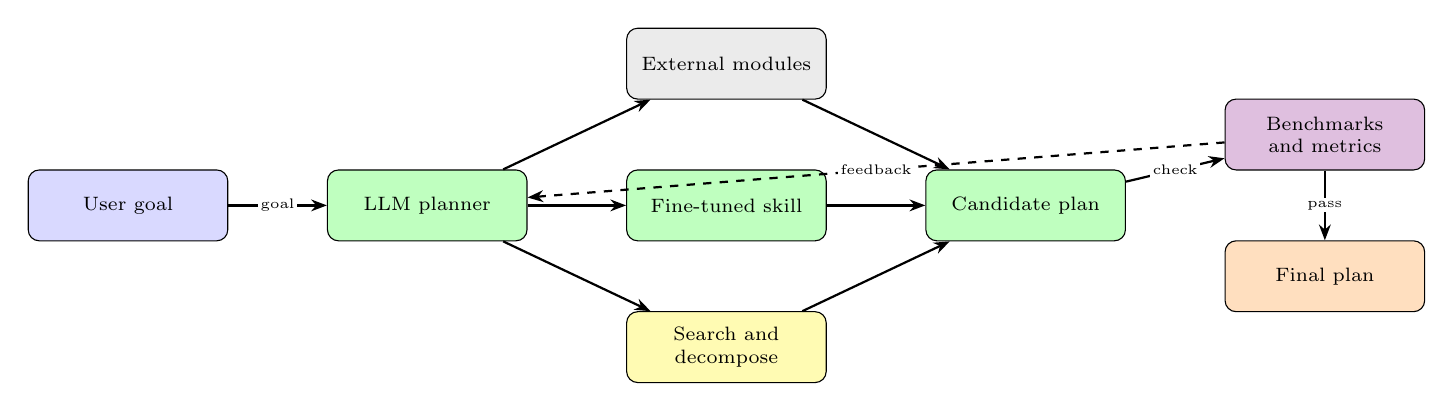
\begin{tikzpicture}
    \node[kuser] (user) at (0.00,0.00) {User goal};
    \node[kagent] (llm) at (3.80,0.00) {LLM planner};
    \node[kdata] (ext) at (7.60,1.80) {External modules};
    \node[kagent] (ft) at (7.60,0.00) {Fine-tuned skill};
    \node[kdecision] (srch) at (7.60,-1.80) {Search and decompose};
    \node[kagent] (plan) at (11.40,0.00) {Candidate plan};
    \node[kguard] (eval) at (15.20,0.90) {Benchmarks and metrics};
    \node[koutput] (out) at (15.20,-0.90) {Final plan};
    \draw[flow] (user) -- (llm) node[midway, font=\tiny, fill=white, inner sep=1pt]{goal};
    \draw[flow] (llm) -- (ext);
    \draw[flow] (llm) -- (ft);
    \draw[flow] (llm) -- (srch);
    \draw[flow] (ext) -- (plan);
    \draw[flow] (ft) -- (plan);
    \draw[flow] (srch) -- (plan);
    \draw[flow] (plan) -- (eval) node[midway, font=\tiny, fill=white, inner sep=1pt]{check};
    \draw[flow] (eval) -- (out) node[midway, font=\tiny, fill=white, inner sep=1pt]{pass};
    \draw[flow, dashed] (eval) -- (llm) node[midway, font=\tiny, fill=white, inner sep=1pt]{feedback};
  \end{tikzpicture}%
  }
  \end{center}
  \begin{center}\scriptsize How an LLM agent turns a user goal into a checked final plan, using three method families with a feedback loop.\end{center}
\end{frame}
\note{This diagram shows the whole flow from left to right. A user gives a goal, the language model interprets it, and then it picks one of the three strategies to produce a draft plan. That plan gets checked against benchmarks and metrics. If it passes it becomes our final answer, and if not, feedback loops back so the model can try again.}
\begin{frame}[allowframebreaks]{How It Works (Explained)}
\begin{itemize}
  \item A user gives the agent a goal written in plain language
  \item The LLM planner interprets that goal and chooses a strategy
  \item It can call external modules, use fine-tuned skill, or search options
  \item These produce a candidate plan: an ordered list of steps
  \item Benchmarks and metrics check the plan for correctness and quality
  \item Passing plans become the final output; failures loop back as feedback
\end{itemize}
\end{frame}
\section{Example Walkthrough}
\begin{frame}[allowframebreaks]{Example Walkthrough: Example: Planning a two-day trip within a budget}
\begin{enumerate}
  \item User asks: plan a two-day Paris trip under 300 dollars
  \item The LLM planner reads the goal and its constraints
  \item It decomposes the goal into subtasks: transport, hotel, meals, sights
  \item It calls tools or memory to fetch prices and options
  \item It assembles an ordered day-by-day plan that fits the budget
  \item A metric checks every constraint is met and each step is valid
  \item If the budget is exceeded, feedback triggers a revised plan
\end{enumerate}
\end{frame}
\note{Let's make this concrete with one simple example. Imagine you ask the agent to plan a two-day Paris trip under three hundred dollars. It breaks the goal into subtasks, looks up prices, and builds a day-by-day plan. Then a check makes sure the budget and other rules are met, revising if needed. That is planning from start to finish.}
\section{Results}
\begin{frame}[allowframebreaks]{Results / Findings}
\begin{itemize}
  \item Survey organizes the field into three families and many sub-methods
  \item TravelPlanner shows the difficulty: GPT-4 passes only 0.6 percent of trips
  \item Classic symbolic tasks like Blocksworld still challenge LLMs planning unaided
  \item Benchmarks span four scenarios: digital, embodied, everyday, and vertical
  \item OpenCodeReasoning dataset covers about 736,000 samples over 28,904 problems
  \item Five metric categories judge correctness, efficiency, consistency, tool use, and interaction
\end{itemize}
\end{frame}
\note{What did we learn from the numbers? The big headline is that planning is genuinely hard. On the TravelPlanner benchmark, GPT-4 succeeds on only about half a percent of trips. The survey also catalogs benchmarks across four kinds of scenarios and five categories of metrics, giving us a full scoreboard of the field.}
\section{Discussion}
\begin{frame}{Discussion}
\begin{itemize}
  \item External modules give reliability but need a formal problem description
  \item Fine-tuning bakes in skill but requires costly training data
  \item Searching finds better plans but costs more compute and time
  \item No single family wins everywhere; the choice depends on the task
\end{itemize}
\end{frame}
\note{So which family should you use? Each has a trade-off. External tools are reliable but need a formal problem description. Fine-tuning builds skill into the model but needs lots of training data. Searching finds better plans but costs more compute. There is no single winner, and it really depends on your task.}
\section{Challenges}
\begin{frame}{Limitations \& Challenges}
\begin{itemize}
  \item LLMs still fail on long-horizon and tightly constrained planning tasks
  \item Methods are hard to compare due to inconsistent benchmarks and setups
  \item Current metrics do not fully capture real-world usefulness of plans
  \item As a survey, it organizes existing work rather than running new experiments
\end{itemize}
\end{frame}
\note{It's important to stay honest about the gaps. LLMs still stumble on long tasks with tight constraints. Comparing methods is hard because benchmarks aren't standardized, and our metrics don't fully capture real-world usefulness. And remember, this is a survey, so it mostly organizes existing work rather than running brand-new experiments.}
\section{Future Work}
\begin{frame}{Future Work}
\begin{itemize}
  \item Build unified benchmarks that allow fair cross-method comparison
  \item Improve efficiency so searching-based planning scales more cheaply
  \item Combine the three families into hybrid planning systems
  \item Strengthen self-feedback so agents reliably correct their own plans
\end{itemize}
\end{frame}
\note{Looking ahead, the authors point to a few exciting directions. We need unified benchmarks so comparisons are fair, and cheaper searching so planning can scale. Combining all three families into hybrid systems is promising, and so is making agents much better at correcting their own mistakes.}
\section{Conclusion}
\begin{frame}{Conclusion}
\begin{itemize}
  \item Planning is a core skill for capable, trustworthy AI agents
  \item LLMs can plan, but reliability remains an open challenge
  \item Three families, external, fine-tuning, and searching, organize the field
  \item This map helps beginners choose and build better planning agents
\end{itemize}
\end{frame}
\note{To wrap up, planning is a foundational skill if we want AI agents we can trust. Language models can plan, but reliability is still an open challenge. The three families give us a clean map of the field. I hope this gives you the vocabulary and the confidence to explore further. Thank you.}
\section{References}
\begin{frame}[allowframebreaks]{References}
  \footnotesize
  \begin{enumerate}
    \item Cao, P., Men, T., Liu, W., Zhang, J., Li, X., Lin, X., Sui, D., Cao, Y., Liu, K., \& Zhao, J. (2025). Large Language Models for Planning: A Comprehensive and Systematic Survey. arXiv:2505.19683.
    \item Xie, J., Zhang, K., Chen, J., et al. (2024). TravelPlanner: A Benchmark for Real-World Planning with Language Agents. arXiv:2402.01622.
    \item Yao, S., Yu, D., Zhao, J., Shafran, I., Griffiths, T. L., Cao, Y., \& Narasimhan, K. (2023). Tree of Thoughts: Deliberate Problem Solving with Large Language Models. arXiv:2305.10601.
    \item Liu, B., Jiang, Y., Zhang, X., et al. (2023). LLM+P: Empowering Large Language Models with Optimal Planning Proficiency. arXiv:2304.11477.
    \item Valmeekam, K., Marquez, M., Sreedharan, S., \& Kambhampati, S. (2023). On the Planning Abilities of Large Language Models: A Critical Investigation. NeurIPS 2023; arXiv:2305.15771.
    \item Hao, S., Gu, Y., Ma, H., et al. (2023). Reasoning with Language Model is Planning with World Model. arXiv:2305.14992.
  \end{enumerate}
\end{frame}
\begin{frame}[plain]
  \begin{center}
    {\Huge Thank You}\\[1em]
    {\large Questions?}
  \end{center}
\end{frame}
\end{document}